\documentclass[english,,man,floatsintext]{apa6}
\usepackage{lmodern}
\usepackage{amssymb,amsmath}
\usepackage{ifxetex,ifluatex}
\usepackage{fixltx2e} % provides \textsubscript
\ifnum 0\ifxetex 1\fi\ifluatex 1\fi=0 % if pdftex
  \usepackage[T1]{fontenc}
  \usepackage[utf8]{inputenc}
\else % if luatex or xelatex
  \ifxetex
    \usepackage{mathspec}
  \else
    \usepackage{fontspec}
  \fi
  \defaultfontfeatures{Ligatures=TeX,Scale=MatchLowercase}
\fi
% use upquote if available, for straight quotes in verbatim environments
\IfFileExists{upquote.sty}{\usepackage{upquote}}{}
% use microtype if available
\IfFileExists{microtype.sty}{%
\usepackage{microtype}
\UseMicrotypeSet[protrusion]{basicmath} % disable protrusion for tt fonts
}{}
\usepackage{hyperref}
\hypersetup{unicode=true,
            pdftitle={Conceptual Hierarchy in Child-Directed Speech},
            pdfkeywords={Conceptual learning, child-directed speech, language and cognition},
            pdfborder={0 0 0},
            breaklinks=true}
\urlstyle{same}  % don't use monospace font for urls
\ifnum 0\ifxetex 1\fi\ifluatex 1\fi=0 % if pdftex
  \usepackage[shorthands=off,main=english]{babel}
\else
  \usepackage{polyglossia}
  \setmainlanguage[]{english}
\fi
\usepackage{graphicx,grffile}
\makeatletter
\def\maxwidth{\ifdim\Gin@nat@width>\linewidth\linewidth\else\Gin@nat@width\fi}
\def\maxheight{\ifdim\Gin@nat@height>\textheight\textheight\else\Gin@nat@height\fi}
\makeatother
% Scale images if necessary, so that they will not overflow the page
% margins by default, and it is still possible to overwrite the defaults
% using explicit options in \includegraphics[width, height, ...]{}
\setkeys{Gin}{width=\maxwidth,height=\maxheight,keepaspectratio}
\IfFileExists{parskip.sty}{%
\usepackage{parskip}
}{% else
\setlength{\parindent}{0pt}
\setlength{\parskip}{6pt plus 2pt minus 1pt}
}
\setlength{\emergencystretch}{3em}  % prevent overfull lines
\providecommand{\tightlist}{%
  \setlength{\itemsep}{0pt}\setlength{\parskip}{0pt}}
\setcounter{secnumdepth}{0}

%%% Use protect on footnotes to avoid problems with footnotes in titles
\let\rmarkdownfootnote\footnote%
\def\footnote{\protect\rmarkdownfootnote}


  \title{Conceptual Hierarchy in Child-Directed Speech}
    \author{true \\ true \\ true}
    \date{}
  
% Manuscript styling
\usepackage{upgreek}
\captionsetup{font=singlespacing,justification=justified}

% Table formatting
\usepackage{longtable}
\usepackage{lscape}
% \usepackage[counterclockwise]{rotating}   % Landscape page setup for large tables
\usepackage{multirow}		% Table styling
\usepackage{tabularx}		% Control Column width
\usepackage[flushleft]{threeparttable}	% Allows for three part tables with a specified notes section
\usepackage{threeparttablex}            % Lets threeparttable work with longtable

% Create new environments so endfloat can handle them
% \newenvironment{ltable}
%   {\begin{landscape}\begin{center}\begin{threeparttable}}
%   {\end{threeparttable}\end{center}\end{landscape}}
\newenvironment{lltable}{\begin{landscape}\begin{center}\begin{ThreePartTable}}{\end{ThreePartTable}\end{center}\end{landscape}}

% Enables adjusting longtable caption width to table width
% Solution found at http://golatex.de/longtable-mit-caption-so-breit-wie-die-tabelle-t15767.html
\makeatletter
\newcommand\LastLTentrywidth{1em}
\newlength\longtablewidth
\setlength{\longtablewidth}{1in}
\newcommand{\getlongtablewidth}{\begingroup \ifcsname LT@\roman{LT@tables}\endcsname \global\longtablewidth=0pt \renewcommand{\LT@entry}[2]{\global\advance\longtablewidth by ##2\relax\gdef\LastLTentrywidth{##2}}\@nameuse{LT@\roman{LT@tables}} \fi \endgroup}

% \setlength{\parindent}{0.5in}
% \setlength{\parskip}{0pt plus 0pt minus 0pt}

% \usepackage{etoolbox}
\makeatletter
\patchcmd{\HyOrg@maketitle}
  {\section{\normalfont\normalsize\abstractname}}
  {\section*{\normalfont\normalsize\abstractname}}
  {}{\typeout{Failed to patch abstract.}}
\makeatother
\shorttitle{Conceptual Hierarchy in CDS}
\author{Kyra Wilson\textsuperscript{1}, Michael C. Frank\textsuperscript{1}, \& Abdellah Fourtassi\textsuperscript{2}}
\affiliation{
\vspace{0.5cm}
\textsuperscript{1} Department of Psychology, Stanford University\\\textsuperscript{2} Department of Computer Science, Aix-Marseille University}
\authornote{
'***The experiment, sample size, exclusion criteria, and the model’s main predictions were preregistered at https://osf.io/942gv/'

'All data and analytic code are available at https://github.com/afourtassi/concepts' 

'None of the authors have any financial interest or a conflict of interest regarding this work and this submission.'


Correspondence concerning this article should be addressed to Abdellah Fourtassi, Postal address. E-mail: abellah.fourtassi@univ-amu.fr}
\keywords{Conceptual learning, child-directed speech, language and cognition}
\usepackage{csquotes}
\usepackage{tipa}
\usepackage[sortcites=false,sorting=none]{biblatex}
\usepackage{tabularx}

\abstract{
``In order for children to understand and reason about the world in a adult-like fashion, they need to learn that conceptual categories are organized in a hierarchical fashion (e.g., a dog is also an animal). The caregiver's linguistic input can play an important role in this learning, and previous studies have documented several cues in parental talk that can help children learn the conceptual hierarchy. However, these previous studies used different datasets and methods which made difficult the systematic comparison of these cues and the study of their relative contribution. Here, we use a large-scale corpus of child-directed speech and a classification-based evaluation method which allowed us to investigate, within the same framework, various cues that vary radically in terms of how explicit the information they offer is. We found the most explicit cues to be too sparse or too noisy to support robust learning. In contrast, the implicit cues offered, overall, a reliable source of information. Our work confirms the utility of caregiver talk for conveying conceptual information. It provides a stepping stone towards a cognitive model that would use this information in a principled way, leading to testable predictions about children's conceptual development.''
}

\begin{document}
\maketitle

\hypertarget{introduction}{%
\section{Introduction}\label{introduction}}

A hallmark of conceptual knowledge is its hierarchical organization. For example, a husky can be categorized as a dog, but it can also be categorized as a mammal, an animal, or a living being. Hierarchical organization is fundamental to human cognition as it allows, among other things, the generalization of knowledge through inference. For example, upon learning that all living beings are made out of cells, one can conclude that dogs are made of cells, too (e.g., Gelman \& O'Reilly, 1988; Markman, 1989).

There are signs that children as young as 3 years old show hierarchical knowledge in various domains (e.g., animals, clothes, and food). Such signs include using superordinate words like \enquote{food} and \enquote{animal} according to parental report (Fenson et al., 1994), using different words to label the same object at different levels of conceptual hierarchy (Clark, 1997), and being able to extend the meaning of novel words to superordinate categories even controlling for perceptual similarity (Liu, Golinkoff, \& Sak, 2001).

How do children acquire conceptual hierarchy? Early accounts considered
conceptual hierarchy to be the consequence of the emergence of a
domain-general logic of class-inclusion -- in other words grasping the idea that one category can be part of a larger one (Inhelder \& Piaget, 2013; Sloutsky, 2015). Children can acquire hierarchy in a specific domain before mastering the domain-general logic of classes, however (Carey, 1987; Chi, Hutchinson, \& Robin, 1989; Inagaki \& Hatano, 2002; Keil, 1981), suggesting that category-specific input may play a role in this development.

Further, a large body of work has focused on children's \emph{sensorymotor} experience to account for the development of hierarchcial knwoldege in a specific domain (e.g., Madole \& Oakes, 1999; McClelland \& Rogers, 2003; Quinn \& Eimas, 2000; Sloutsky, 2010; Smith \& Heise, 1992). For example, children may learn that \enquote{pigeon} and \enquote{raven} are both members of the same category because they look similar. However sensorymotor experience is not the only source of information people use to glean conceptual knowldege. A striking example is the fact that \enquote{visual} semantic knowledge in congenitally blind individuals is very similar to that of sighted individuals (e.g., Kim, Elli, \& Bedny, 2019; Lewis, Zettersten, \& Lupyan, 2019).

In addition, sensorymotor experience alone may not be suffisant to account for the entire richeness of taxonomic knowldedge: Instances of superordinate categories do not necessarily share similar --- sensory accessible --- features, and their learning may require addtional, culture-specifc information. For example, the categories \enquote{animal} and \enquote{plants} are organized for Groote Eylandt Australian aborigines into three categories: \enquote{biological}, \enquote{food}, and \enquote{totemic} (Waddy, 1982). Thus children may need additional input, beyond senseory data, to learn about sthe uperordinate categories of their linguistic community.

Previous research has shown that children also learn about the world fom the \emph{language} they hear around them for language can provide children with information beyond what they can obtain through sensorimotor experience alone, especially when learning about categories beyond the here and now such as abstract entities (Csibra \& Gergely, 2009; Gelman, 2009; Harris, 2012).

Following this research, the current study tests the extent to which child-directed speech cantains cues that could help children learn conceptual hierarchy. Some previous studies analyzed parent-child interactions and observed that when parents introduce words at the superordinate level, they typically also provide the basic level term (Blewitt, 1983; Callanan, 1985; Shipley, Kuhn, \& Madden, 1983). For example, parents rarely point to an object and say \enquote{this is an animal!} Instead, they usually \emph{anchor} the superordinate word \enquote{animal} at the basic level by saying something along the lines of \enquote{This is a duck; a duck is a kind of animal.} Such an anchoring strategy provides children with a categorization of the same object at different levels, which may help children understand the underlying hierarchical organization.

More recent research, prompted by advances in machine learning (Landauer \& Dumais, 1997; Mikolov, Sutskever, Chen, Corrado, \& Dean, 2013), found that the statistical distribution of basic-level terms in parental speech can lead to coherent structures at the superordinate level (Fourtassi, Scheinfeld, \& Frank, 2019, Frermann and Lapata (2016); Huebner \& Willits, 2018). For example, though \enquote{fish} and \enquote{bird} do not look very similar, people talk about them in similar linguistic contexts, typically leading to a similar distributions in speech. Having a shared pattern of co-occurrence (i.e., a shared distribution) can cue taxnomic relationship (e.g., Sloutsky, Yim, Yao, \& Dennis, 2017). Such distributional information can be a powerful source of conceptual knowledge because it does not require the presence of a lexicalized label for the higher-level category. On this kind of account, categories emerge in a bottom-up fashion as a cluster of related words at the lower-level.

The lingusitic cues reviewed above can be thought of as ends in a continuum that varies from explicit to implicit. The \enquote{is-a-kind-of} cue is the most explicit cue since both the terms (i.e., the basic and superordinate labels) and their hierarchical relationship are explicitly stated. The pure distributional cue is the most implicit cue since, on the one hand, the superordinate term is not required and, on the other hand, the hierarchical relationship (that is, the fact that co-occurring basic level terms are part of a higher-level category) can only be induced.

While previous studies have focused on these extremes, other cues are available that have an intermediate status on this continuum. Here, we examine the way parents hint at the hierarchical relationship between two concepts pragmatically without using an explicit inclusion expression. For example, instead of saying \enquote{a cow is a kind of animal} parents can say the following (e.g., in the context of a play session): \enquote{Do you want a cow or do you want another animal?} (see Table 1 for more examples). We also study whether action affordances provide another -- perhaps more implicit -- cue for category membership. For example, food items could be identified as members of a category by virtue of their compatibility with the verb \enquote{eat} and clothing items by their compatibility with \enquote{wear.} (see Figure \ref{fig:cues}).

\begin{figure}[h]

{\centering 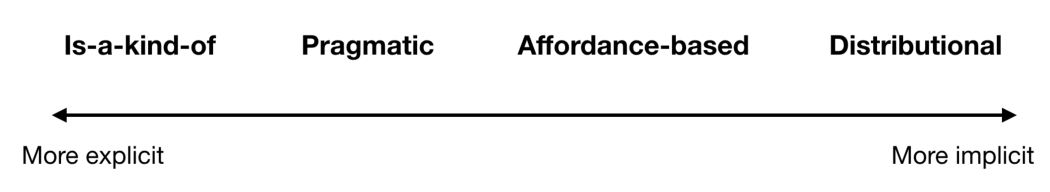
\includegraphics{cogsci_journal_files/figure-latex/cues-1} 

}

\caption{\label{fig:cues} The cues to conceptual hierachy in the lingusitic input can be understood as falling on a continuum from most explicit to most implicit.}\label{fig:cues}
\end{figure}

\hypertarget{this-study}{%
\subsection{This study}\label{this-study}}

Previous studies examining individual cues to categorization vary in terms of both the datasets and methods they used, which has made comparison difficult. Implicit cues have
generally been studied using large-scale data and have been evaluated based on their ability to provide an accurate similarity space for words. In contrast, explicit cues have been studied mainly in the context of small-scale experiments and have been tested mainly through counting the frequency of a given linguistic expression (e.g., \enquote{X is a kind of Y}).

In this work, we make a systematic comparison of explicit and implicit cues using similar methods. In particular, we are interested in quantifyong the infromation provided by each of these cues in spontaenous (rather than scripted) child-directed sppech, using language data from naturalistic child-caregiver interactions (CHILDES 2018.1, MacWhinney, 2000; Sanchez et al., 2019), tested across the entire normative vocabulary. Such comparison is crucial as it allows us, for instance, to formualte hypotheses about the relative role each cue could play in development and about the ability of these cues to scale up to naturalistic data.

To this end, we take a classification approach: We operationalize different cues as features that can be used to compute similarity. We then evaluate this continuous similarity measure by using it for a classification task, deciding whether different basic-level categories are part of the same superordinate category. Thus we can assign a classification accuracy to each cue type.

The paper is organized as follows. We begin by introducing our child-directeed data and the set of conceptual cues we consider. We then exlain the task and evaluation methods that we use to study and compare the cues. Next, we present the results quantifying the role of each of the four cues and their relative informativeness across development. Finally we discuss our findings in the light of the litterature on early linguistic and conceptaul development.

\hypertarget{analyses}{%
\section{Analyses}\label{analyses}}

\hypertarget{data}{%
\subsection{Data}\label{data}}

We constructed a large-scale corpus by aggregating over all English-language transcripts from CHILDES (MacWhinney, 2000; Sanchez et al., 2019). We selected all utterances in which the speaker was not tagged as \enquote{Child} or \enquote{Target\_Child} and which were addressed to children up to three years of age. The final corpus contained 1.9 million utterances and 7.9 million words from a collection of 4,939 transcripts across 660 children with an average age of 26.8 months.

We decided to study the six following superordinate categories: \enquote{animal}, \enquote{furniture}, \enquote{clothes}, \enquote{food}, \enquote{toys} and \enquote{vehicles}. For each of these categories, we used the corresponding basic-level terms available in the English-language MacArthur-Bates Communicative Inventory (CDI) (Fenson et al., 1994), a parent-report instrument that provides a partial listing and categorization of words produced by children 18--30 months. This set of categories was chosen because it combines all sets of
superordinate categories that had been studied previously and for which CDI data were available. Indeed, most previous experimental work (which we partly reviewed above) used only a subset of these categories for a given study. Further, a Data-driven approach using CDI words and input from CHILDES (Fourtassi et al., 2019) led a set of categories made of: \enquote{animal}, \enquote{food,} \enquote{clothes,} and a broad category of \enquote{artifacts} which included instances of toys, vehicles, and furniture. Here, we kept the last three categories differentiated as in previous experimental work.

\hypertarget{cues-to-conceptual-hierarchy-and-their-feature-vectors}{%
\subsection{Cues to Conceptual Hierarchy and their Feature Vectors}\label{cues-to-conceptual-hierarchy-and-their-feature-vectors}}

As indicated above, we explored four cues to conceptual hierarchy: \enquote{is-a-kind-of}, pragmatic, verb affordance-based, and distributional.
We represented each cue as a set of features and we tested how these features allow us to classify basic-level terms into superordinate
categories. To this end, we started by using each cue to derive a feature vector for each basic-level word in the CDI lexicon. In the case where the cue relied on an explicit category marker (i.e., the first three cues), the feature vectors were based on the superordinate categories introduced above. Otherwise (e.g., the fourth cue), the feature vector was an embedding in a high dimensional space derived based on the words' shared pattern of co-occurrence only. In the following, we explain how we computed the feature vectors for each cue (see also Figure \ref{fig:task}).

\hypertarget{is-a-kind-of}{%
\subsubsection{Is-a-kind-of}\label{is-a-kind-of}}

This cue tests the extent to which parents use explicit expressions of class inclusion (Callanan, 1985). For each word at the basic label, X,
we construct a feature vector of length 6, where every cell corresponds to a superordinate category, Y, and the entry in each cell corresponds to the frequency with which X appears with Y is in one of the following expressions: \enquote{X is a/an Y} or \enquote{X is a kind/type/sort of Y} (we kept the same expressions used in previous studies).

\hypertarget{pragmatic}{%
\subsubsection{Pragmatic}\label{pragmatic}}

Parents can express conceptual hierarchy between X and Y without
necessarily using an \enquote{is-a-kind-of} expression. In many cases, parents
can hint at this hierarchy using a wide diversity of
linguistic expressions (Table 1). Detecting these expressions at scale is a challenge given their complexity, so as a first attempt to capture this diversity, we relax
grammatical constraints between X to Y, and we keep only the requirement
that X and Y should co-occur.

More concretely, we represent each basic-level term, X, with a feature
vector where each entry represents the frequency with which X co-occurs
with the corresponding superordinate term Y. This co-occurrence is
determined using a fixed window of \(k\) utterances. Values of \(k > 1\)
allow us to capture the case where a relationship between X and Y is
established across more than one utterance. For example:

-- Mother : What kind of animal is this?

-- Mother : It's a giraffe!

\begin{table}[!htbp] \centering 
\begin{tabularx}{\linewidth}{cXXc}
\hline
\textbf{Category} & Utterance & Interlocutors & Corpus\\
\hline

\textbf{Animals} & Do you want a cow or do you want a different animal? & Mother to Max, 30 months & EllisWeismer\\

\textbf{Furniture} & Furniture means sofas and chairs and... & Mother to Naima, 23 months & Providence\\

\textbf{Clothes} & This is another clothes. See it's just like this shirt. & Investigator to Shem, 30 months & Clark\\

\textbf{Food} & She asked Lily what her favorite food was. If Lily says chocolate I am in trouble. & Mother about Lily, 24 months & Providence\\

\textbf{Toys} & You close the book and we'll get a different toy cause I think you're tired of this. & Mother to child, 13 months & Ambrose\\

\textbf{Vehicles} & The only vehicle you cut out so far is the train. & Mother to Warren, 30 months & Manchester\\

\hline
\end{tabularx}
\caption{\label{tab:pragmatic} Examples of utterances from CHILDES where parents hint at a hierachical relations between basic- and superordinate- level terms.}
\end{table}

\hypertarget{affordance-based}{%
\subsubsection{Affordance-based}\label{affordance-based}}

The super-ordinate label is not the only category marker that can cue conceptual hierarchy for a basic level term, especially when this category can be characterized by an affordance. For example, \enquote{food} can be characterized as the category of things we eat and \enquote{clothes} as things we wear. Thus, children can learn that some concepts (e.g., \enquote{apple} and \enquote{bread}) are parts of a higher-level category (\enquote{things we eat}) by observing how these concepts co-vary with a cue of their common affordance (i.e., the verb \enquote{eat}).

We computed the feature vectors for this cue as follows. In a first step, we tried to find a verb that could be used as an affordance marker for an entire category. We used \enquote{eat} for food, \enquote{wear} for clothes, \enquote{play} for toys, and \enquote{ride} for vehicles. The category \enquote{furniture} has no such obvious function verb. We decided to use the verb \enquote{use} because if there were a verb that could fit every member of the category of furniture, it would be that (even though it can also fit things that are not members of the category). For the animal category, we could find no verb that could categorize the instances.

In addition to these verbs, we also identified synonymous verbs for each category that could also signifiy an affordance for the category. However, these verbs were either not found in the corpus (words like \enquote{devour} and \enquote{utilize} are not used in child directed speech) or they occurred in too many contexts to be useful for categorization (\enquote{have} can be used synonymously with \enquote{eat}, but it has additional meanings that make this not a useable cue). Because of this, only one verb was used for computing the feature vectors for each of the categories.

We detected the concept-affordance relationship, syntactically, based on their occurrence in a verb-complement structure.\footnote{There are more complex structures that could, in principle, be used by parents. We used the simplest as a first approximation, though the performance of this cue could likely be enhanced by considering a wider variety of constructions.} For example, in the utterance \enquote{the bird eats the berries}, the word \enquote{berries} was categorized as \enquote{eat}-able. For each basic-level term, we computed a feature vector where entries correspond to the frequency with which this term occurs in a verb-complement relationship with the verb/affordance at hand.

\hypertarget{distributional-cue}{%
\subsubsection{Distributional cue}\label{distributional-cue}}

Unlike the first three cues, the pure distributional cue is not based on an explicit category marker at the superordinate level. It is based,
instead, on the way basic-level terms are distributed together in speech (Harris, 1957). Following previous research (Fourtassi et al., 2019), we quantified this cue using the word embedding model Word2Vec (Mikolov et al., 2013). We used this model to represent basic-level words as vectors in a high-dimensional space, representing the distribution of these words in a latent semantic structure.

\hypertarget{task-and-evaluation}{%
\subsection{Task and Evaluation}\label{task-and-evaluation}}

Above, we characterized all cues in a vectorial framework. This
framework allows us to directly compare the cues in terms of how they
quantify the similarity between words (defined as the cosine of the
angle formed by their vectors). Based on this similarity, we test the
ability of each cue to predict which pairs of words (from the normative vocabulary) belong to the same superordinate category (e.g., \enquote{apple} and \enquote{bread}) and which pairs
of words belong to different categories (e.g., \enquote{apple}, \enquote{horse}).

We listed all pairs of basic-level words in the CDI dataset and their cosine similarity (according to each cue). Then, we evaluated the ability of the similarity measures to accurately predict whether the pairs belonged to \enquote{same} or \enquote{different}
categories, across the full range of possible discrimination thresholds.
We quantified performance in the task using the standard Area Under the ROC curve (hereafter AUC). The AUC score can be interpreted as the probability that, given two pairs of words, of which one is from the same category, the pairs are correctly classified based on the similarity. For each cue, we derived both a global AUC score across all
categories and a category-specific AUC score where we evaluated only the
subset of pairs of words that contained at least an instance of a target
category (see Figure \ref{fig:task}).\footnote{A similar task and evaluation method have been used in previous work to evaluate cues to phonological categories in early development (Fourtassi, Dunbar, \& Dupoux, 2014; Fourtassi \& Dupoux, 2013).}

\begin{figure}[h]

{\centering 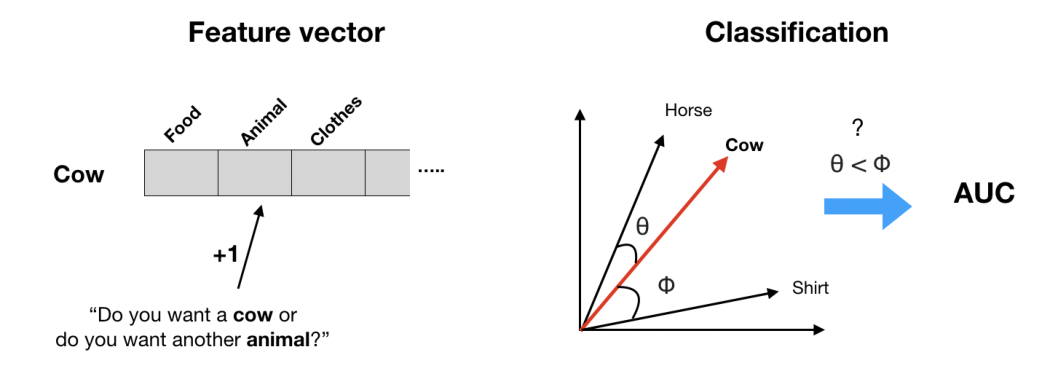
\includegraphics{cogsci_journal_files/figure-latex/task-1} 

}

\caption{\label{fig:task} A schematic description of the task. For each basic-level word (here, `cow') a feature vector is derived from child-directed speech based on how the cue is defined. Here, the vector cells correspond to the superordinate categories. The entry in a given cell (e.g., animal) is incremented when the word `cow' co-occurs with the corresponding category label. The cue is evaluated based on its ability to classify pairs of words into 'same' or 'different' superordinate categories. Here, the pair `cow'-`horse' belongs to the same category. The corresponding vectors should be closer to each other than the vectors of a pair that belongs to different categories (e.g., `cow'-`shirt'). This evaluation is quantified by a standard measure in signal detection theory called the Area Under the ROC Curve (AUC).}\label{fig:task}
\end{figure}

\hypertarget{results}{%
\section{Results}\label{results}}

\hypertarget{individual-cue-results}{%
\subsection{Individual Cue Results}\label{individual-cue-results}}

Instances of our most explicit cue type, the \emph{\enquote{is-a-kind-of} cue}, were so rare that we could not even build feature vectors for basic-level words. In total, we found only four instances, all of them characterizing the \enquote{animal} category. Thus, we did not have meaninful results to report for this cue. As for the other cues, Figure \ref{fig:data-all} shows the global AUC score across categories as well as the AUC scores specific to each category.

\begin{figure}[h]

{\centering 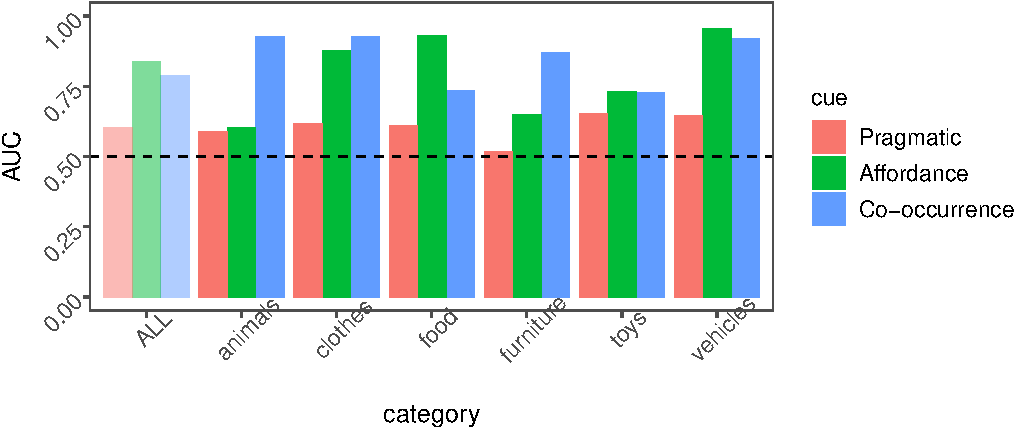
\includegraphics{cogsci_journal_files/figure-latex/data-all-1} 

}

\caption{\label{fig:data-all} The Area Under the ROC Curve (AUC) scores of the cues for each category and across all categories ('ALL'). A value of 0.5 represents pure chance, and a value of 1 represents perfect performance. The AUC score can be interpreted as the probability that, given two pairs of basic-level words, of which one is from the same superordinate category, the pairs are correctly classified using their  cue-based similarity.}\label{fig:data-all}
\end{figure}

The accuracy of the \emph{pragmatic cue} was generally low. For this cue, we only report the results with \(k=1\), which captures relations between basic and superrodinate words within a single utterance. Increasing the value of \(k\) lead to worse, noisier performance. Regarding the \emph{affordance-based cue}, the accuracy was relatively high for some categories, i.e., \enquote{food}, \enquote{clothes}, \enquote{vehicles}, and \enquote{toys} and low for others, i.e., \enquote{furniture} and \enquote{animal.} Finally, the \emph{distributional cue} lead to the best overall results across most superordinate categories.

\hypertarget{developmental-change}{%
\subsection{Developmental change?}\label{developmental-change}}

The results we showed concern cues derived from parental speech to children up to 3
years old, as this is the age when signs of conceptual hierarchy start
to emerge in the developmental literature. But we were also interested
in how information in these cues may change as children grow older.
For this analysis, we followed the same approach as above but included progressively more data in the corpus by adding utterances addressed to older children (Table \ref{tab:development}). Results of this analysis, presented in Figure \ref{fig:dev}, show that the performance of all cues remained stable across development, at least up to 6 years old.

\begin{table}[!htbp] \centering 
\begin{tabularx}{\linewidth}{cXccXX}

\textbf{Age} & Age (months) & Children & Transcripts & Utterances & Words \\
\hline

\textbf{\textless4} & 30.1 & 843 & 6,750 & 2.657 M & 10.827 M\\

\textbf{\textless5} & 33.5 & 971 & 7,889 & 3.093 M & 12.807 M\\

\textbf{\textless6} & 34.8 & 1,046 & 8,654 & 3.221 M & 13.325 M\\

\hline
\end{tabularx}
\caption{\label{tab:development} Information about the corpora used in the analysis of developmental change.}
\end{table}

\begin{figure}[!htbp]

{\centering 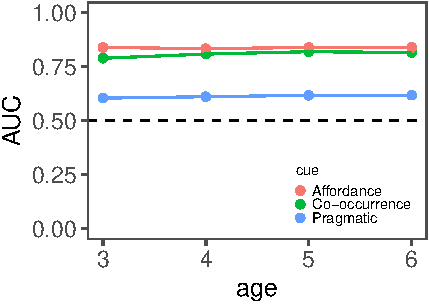
\includegraphics{cogsci_journal_files/figure-latex/dev-1} 

}

\caption{\label{fig:dev} The Area Under the ROC Curve (AUC) scores for each cue (across all categories) using speech heard by children up to a particular age. A value of 0.5 represents pure chance, and a value of 1 represents perfect performance.}\label{fig:dev}
\end{figure}

\hypertarget{cross-cue-results}{%
\subsection{Cross-cue results}\label{cross-cue-results}}

Here we explored the extent to which explicit and implicit cues provided
complementary vs.~redundant information. To this end, we fit logistic
regressions predicting the binary classification of pairs of basic-level
words as belonging to same or different superordinate categories. The
predictors were the pairs' similarity measures derived from each cue (centered and scaled to maximize comparability; the is-a-kind-of cue was not included due to sparsity). The results of the regressions,
summarized in Table \ref{tab:regressions}, indicate that, overall, each cue remains highly significant when controlling for the other cues. Thus, although distributional cues were highest performing when alone, each cue type provided \emph{non-redundant} information and the overall classification performance increased when multiple information sources were used.

\begin{table}[!htbp] \centering 
\caption{\label{tab:regressions} Logistic regressions predicting the binary classification of pairs of basic-level words as belonging to same or different superordiante categories. The predictors are the pairs' similarity measures derived from each cue. We fit a different regression for each superodinate category.} 
\label{} 
\begin{tabular}{@{\extracolsep{5pt}}lcccccc} 
\hline 
 & \multicolumn{4}{c}{} \\
 & (Intercept) & Distributional & Affordance & Pragmatic \\ 
\hline \\[-1.8ex] 
  Animals & $-$2.741$^{***}$ & 2.285$^{***}$ & 0.022 & 0.179$^{***}$\\
  & (0.085) & (0.074) & (0.057) & (0.050)\\
  & & & & & & \\
  Furniture & $-$3.195$^{***}$ & 2.040$^{***}$ & 0.547$^{***}$ & $-$0.104\\
  & (0.138) & (0.127) & (0.094) & (0.080) &\\
  & & & & & & \\
  Toys & $-$3.244$^{***}$ & 1.178$^{***}$ &  0.620$^{***}$ & 0.722$^{***}$\\
  & (0.155) & (0.136) & (0.113) & (0.120) &\\
  & & & & & & \\
  Food & $-$2.616$^{***}$ & 0.905$^{***}$ & 2.112$^{***}$ & 0.325$^{***}$\\
  & (0.112) & (0.060) & (0.092) & (0.059)\\
  & & & & & & \\
  Clothing & $-$3.101$^{***}$ & 1.644$^{***}$ & 1.535$^{***}$ & 0.359$^{*}$\\
  & (0.183) & (0.171) & (0.153) & (0.146)\\
  & & & & & & \\
  Vehicles & $-$4.663$^{***}$ & 1.249$^{***}$ & 2.211$^{***}$ & 0.159\\
  & (0.348) & (0.193) & (0.245) & (0.138)\\
  & & & & & & \\
 \\[-1.8ex] 

\hline \\[-1.8ex] 
\textit{Note:}  & \multicolumn{6}{r}{$^{*}$p$<$0.05; $^{**}$p$<$0.01; $^{***}$p$<$0.001} \\ 
\end{tabular} 
\end{table}

\hypertarget{discussion}{%
\section{Discussion}\label{discussion}}

A crucial questions in the study of cogntive developemnt is understanding how children acquire the complex hierarchical relationships that characterize mature human conceptual knowledge. A particualrly challenging task is learning how basic-level categories are grouped into abstract superordinate categories. The difficulty of this task stems form the fact that sensorimotor experience does not always provide direct evidence for learning. Here we build on and extend previous work investigating the role of \emph{language} in learning about abstract concepts (Csibra \& Gergely, 2009; Gelman, 2009; Harris, 2012). The novelty of our work is that we used a unified computational framework that has allowed us to directly compare the relative importance of different linguistic cues present in child-directed speech with respect to their ability to help categorize six common superordinate categories. Overall, we found that caregiver talk provides a rich source of information, especially in its implcit form, that chidlren may use in learning category structure.

The most explicit cue --- where caregivers state the relationship between a basic-level term and its superordiante category label (e.g., \enquote{a dog is a kind of animal}) --- did not scale up well to the naturalistic dataset we used. This finding contrasts with previous work that found this cue in parental speech (Blewitt, 1983; Callanan, 1985; Shipley et al., 1983). This contrast can be explained by the fact that these previous studies were done in the context of rather controlled settings and parents were aware of the task (e.g., teaching words at the superordinate level), whereas here we tested a large-scale corpus containing a diversity of situations. Thus, it is possible that, in these previous studies, parents used a teaching strategy that they thought could optimize the short-term outcome (as determined by the experimenter), rather than a strategy that reflects their spontaneous interaction with children in daily life.

Caregivers can hint at conceptual hierarchy without necessarily stating it explcitly, however (Table 1). To capture this pragmatic cue, we quantified the co-occurrence between basic-level and superordinate terms within utterances. While this simple operationalization was ment to capture all possible ways the hierarchical relation between two concepts can be expressed linguistically, it also made the representation susceptible to errors, mainly by increasing the rate of false alarms: A basic level term (e.g., \enquote{juice}) can also co-occur with a superordinate label of which it is not an instance (e.g., \enquote{Don't pour the juice on your clothes!}). The rate of such false alarms was quite high, which explaines to overall low --- though not random --- scores of this cue. From a developmental point of view, this finding highlights the limitation (at scale) of a simple co-occurrence-based strategy: A deeper understanding of the utterance is necessary if chidlren are to learn conceptual hierachy from pragmatic cues while avoiding false alarms. Future work can aim at quantifying such deeper understansing. That said, this is not an easy task since an \emph{automatic} method that ``understands'' how words are related both semantically and pragmatically is an open computational questions.

Another lingustic cue was based on verb affordance (e.g., basic-level terms for food can all occur as the grammatical objet of the verb \enquote{eat}). The acccuracy of the affrodance-based cue was relatively high for the categories which had an obvious verb to cue its affordance, i.e., \enquote{food} (eat), \enquote{clothes} (wear), \enquote{vehicles} (ride), and \enquote{toys} (play). The accuracy was low in the case of \enquote{furniture} since the verb \enquote{use} is not exclusive to this category and can also be used with instances of other categories, leading to false alarms. The accuracy for
\enquote{animal} was also low as it was not characterized by any particular affordance verb. \footnote{At the same time, performance of the cue on this category was not totally random as animal instances tend to co-occur consistently with some verbs from other categories (e.g., "ride a horse", "play with the dog", and "eat the chicken").}

The distributional cue was the most implicit one since it did not require a label for the abstract category. The score for this cue was generally high, including for \enquote{animal} and \enquote{furniture}, two categories that were not accurately captured with any of the previous
cues. This finding suggests that children can learn that certain basic-level terms share common abstract properties by realizing that they have similar distribution in speech, i.e., that they are used in similar contexts. This strategy seems even more plausible for high-level categories that do not have an explicit label, or for which the label could not be available to the young learners (e.g., \enquote{animate} vs. \enquote{inanimate}).

An important finding was that the linguistic cues were largely non-redundant across the categories, suggesing that children can combine several cues to refine their knowlwdege about superordinate concepts. In addition, the cues did not fare similarly across categories, suggesting that children can rely more on different cues to learn different categories, e.g., they may use the affordance-based cue more to learn about \enquote{food}, \enquote{clothes} or \enquote{vehilce} and the distributional cue more to learn about \enquote{animals} and \enquote{furniture.}

For all the cues discussed above, our goal was to test their ability to provide a reliable source of information in child-directed speech. However, our instantiation of the cues abstracted aways the children's cognitive and informaton processsing limitations, providing only an \enquote{ideal observer} point of view (Marr, 1982). That said, previous experimental work have provided evidence for the cognitive plausivility of the learning mechanisms that underly each of these cues.

For instace, preschool children ably use the \enquote{is-a-kind-of} cue to interpret the meaning of a novel word at the superordinate level (Callanan, 1989) (though the current study shows this cue not to be pervasive in the natural input). Both the pragamtic cue and affordance-based cue rely on the ability to track co-occurrence between pairs of words. Extensive research in the last couple of decades has shown that even infants are capable of tracking distributional statistics of various linguistic units (Saffran, Aslin, \& Newport, 1996). In particular, Bannard \& Matthews (2008) have shown toddlers encode together in memory collocational words such as \enquote{sit} and \enquote{chair} and Wojcik \& Saffran (2015) have shown that they encode relationships between novel words co-occurring in a sentence. Previous work also provided evidence showing that patterns of co-occurrence do influence children's conceptual associations and inference (Fisher, Matlen, \& Godwin, 2011; Matlen, Fisher, \& Godwin, 2015).

The distributional cue requires not only sensititvity to co-occurrence, but also sensitivity to their \emph{shared} patterns of co-occurrence. For example, learners should be sensitive to the fact that \enquote{ravin} and \enquote{salmon} co-occur with similar words and phrases such as \enquote{lay egg}, \enquote{live,} and \enquote{reproduce}, although the pair of words \enquote{ravin} and \enquote{salmon} may not themelves co-occur with each other. There is evidence that even infants are sensitive to shared patterns of co-occurrence (e.g., Lany \& Saffran (2011)), although the mechanism by which this sensitivity shapes concptual knowledge emerges slowly and continues developing through middle childhood (see review by Unger \& Fisher, 2021).

This work takes a first step towards integrating different cues to conceptual hierachy from caregiver language. Future work should go further by also considering the role of sensorymotor data (Andrews, Frank, \& Vigliocco, 2014; Bruni, Tran, \& Baroni, 2014; Sadeghi, McClelland, \& Hoffman, 2015). Ultimately, the goal would be to integrate both sources in a \emph{cognitive} model that uses these cues in a principle way. Such a model should make precise developmental predictions about how the cues interact and how their role in learning changes across development.

Another direction for future work is to compare the findings we obtained with data in English to other languages. Understanding variation in children's experience allows us to detrmine which apects of development are universal and which are culture-specific (Medin, Bennis, \& Chandler, 2010; Rogoff, Dahl, \& Callanan, 2018). The case of learning abstract, superodinate categories is an excellent case where such comparison could be very enlightning as we know such categories have both similaritis and differences across cultures (e.g. Waddy (1982)). Thus, it is crucial that we investigate whether and how variation in caregivers' language induce variations in children's categorical structure of the world.

To conclude, our work here suggests the presence of multiple information sources about conceptual structure in children's linguistic environment. Perhaps the most exciting future direction is to synthesize it with knowledge gleaned from children's sensory experience of the world. Such a synthesis will be crucial in making progress on understanding children's conceptual structure. By refining our understanding of linguistic cues to conceptual hierarchy, we hope our work here helps take a first step in this broader project.

\hypertarget{references}{%
\section{References}\label{references}}

\setlength{\parindent}{-0.5in}
\setlength{\leftskip}{0.5in}

\hypertarget{refs}{}
\leavevmode\hypertarget{ref-andrews2014}{}%
Andrews, M., Frank, S., \& Vigliocco, G. (2014). Reconciling embodied and distributional accounts of meaning in language. \emph{Topics in Cognitive Science}, \emph{6}(3), 359--370.

\leavevmode\hypertarget{ref-bannard2008}{}%
Bannard, C., \& Matthews, D. (2008). Stored word sequences in language learning: The effect of familiarity on children's repetition of four-word combinations. \emph{Psychological Science}, \emph{19}(3), 241--248.

\leavevmode\hypertarget{ref-blewitt1983}{}%
Blewitt, P. (1983). Dog versus collie: Vocabulary in speech to young children. \emph{Developmental Psychology}, \emph{19}(4).

\leavevmode\hypertarget{ref-bruni2014}{}%
Bruni, E., Tran, N.-K., \& Baroni, M. (2014). Multimodal distributional semantics. \emph{Journal of Artificial Intelligence Research}, \emph{49}, 1--47.

\leavevmode\hypertarget{ref-callanan1985}{}%
Callanan, M. A. (1985). How parents label objects for young children: The role of input in the acquisition of category hierarchies. \emph{Child Development}, 508--523.

\leavevmode\hypertarget{ref-callanan1989}{}%
Callanan, M. A. (1989). Development of object categories and inclusion relations: Preschoolers' hypotheses about word meanings. \emph{Developmental Psychology}, \emph{25}(2).

\leavevmode\hypertarget{ref-carey1987}{}%
Carey, S. (1987). \emph{Conceptual change in childhood}. MIT Press.

\leavevmode\hypertarget{ref-chi1989}{}%
Chi, M. T., Hutchinson, J. E., \& Robin, A. F. (1989). How inferences about novel domain-related concepts can be constrained by structured knowledge. \emph{Merrill-Palmer Quarterly (1982-)}, 27--62.

\leavevmode\hypertarget{ref-clark1997}{}%
Clark, E. V. (1997). Conceptual perspective and lexical choice in acquisition. \emph{Cognition}, \emph{64}(1), 1--37.

\leavevmode\hypertarget{ref-csibra2009}{}%
Csibra, G., \& Gergely, G. (2009). Natural pedagogy. \emph{Trends in Cognitive Sciences}, \emph{13}(4), 148--153.

\leavevmode\hypertarget{ref-fenson94}{}%
Fenson, L., Dale, P. S., Reznick, J. S., Bates, E., Thal, D. J., Pethick, S. J., \ldots{} Stiles, J. (1994). Variability in early communicative development. \emph{Monographs of the Society for Research in Child Development}, \emph{59}(5), i--185.

\leavevmode\hypertarget{ref-fisher2011}{}%
Fisher, A. V., Matlen, B. J., \& Godwin, K. E. (2011). Semantic similarity of labels and inductive generalization: Taking a second look. \emph{Cognition}, \emph{118}(3).

\leavevmode\hypertarget{ref-fourtassi2014}{}%
Fourtassi, A., Dunbar, E., \& Dupoux, E. (2014). Self-consistency as an inductive bias in early language acquisition. In \emph{Proceedings of the annual meeting of the cognitive science society} (Vol. 36).

\leavevmode\hypertarget{ref-fourtassi2013}{}%
Fourtassi, A., \& Dupoux, E. (2013). A corpus-based evaluation method for distributional semantic models. In \emph{51st annual meeting of the association for computational linguistics proceedings of the student research workshop} (pp. 165--171).

\leavevmode\hypertarget{ref-fourtassi2019}{}%
Fourtassi, A., Scheinfeld, I., \& Frank, M. C. (2019). The development of abstract concepts in children's early lexical networks. In \emph{Proceedings of the workshop on cognitive modeling and computational linguistics} (pp. 129--133).

\leavevmode\hypertarget{ref-frermann2016}{}%
Frermann, L., \& Lapata, M. (2016). Incremental bayesian category learning from natural language. \emph{Cognitive Science}, \emph{40}(6), 1333--1381.

\leavevmode\hypertarget{ref-gelman2009}{}%
Gelman, S. A. (2009). Learning from others: Children's construction of concepts. \emph{Annual Review of Psychology}, \emph{60}, 115--140.

\leavevmode\hypertarget{ref-gelman1988}{}%
Gelman, S. A., \& O'Reilly, A. W. (1988). Children's inductive inferences within superordinate categories: The role of language and category structure. \emph{Child Development}, 876--887.

\leavevmode\hypertarget{ref-harris2012}{}%
Harris, P. L. (2012). \emph{Trusting what you're told}. Harvard University Press.

\leavevmode\hypertarget{ref-harris1957}{}%
Harris, Z. S. (1957). Co-occurrence and transformation in linguistic structure. \emph{Language}, \emph{33}(3).

\leavevmode\hypertarget{ref-huebner2018}{}%
Huebner, P. A., \& Willits, J. A. (2018). Structured semantic knowledge can emerge automatically from predicting word sequences in child-directed speech. \emph{Frontiers in Psychology}, \emph{9}, 133.

\leavevmode\hypertarget{ref-inagaki2002}{}%
Inagaki, K., \& Hatano, Giyoo. (2002). \emph{Young children's naive thinking about the biological world}. New York : Psychology Press.

\leavevmode\hypertarget{ref-inhelder2013}{}%
Inhelder, B., \& Piaget, J. (2013). \emph{The early growth of logic in the child: Classification and seriation}. Routledge.

\leavevmode\hypertarget{ref-keil1981}{}%
Keil, F. C. (1981). Constraints on knowledge and cognitive development. \emph{Psychological Review}, \emph{88}(3).

\leavevmode\hypertarget{ref-kim2019}{}%
Kim, J. S., Elli, G. V., \& Bedny, M. (2019). Knowledge of animal appearance among sighted and blind adults. \emph{Proceedings of the National Academy of Sciences}, \emph{116}(23), 11213--11222.

\leavevmode\hypertarget{ref-landauer1997}{}%
Landauer, T. K., \& Dumais, S. T. (1997). A solution to plato's problem: The latent semantic analysis theory of acquisition, induction, and representation of knowledge. \emph{Psychological Review}, \emph{104}(2).

\leavevmode\hypertarget{ref-lany2011}{}%
Lany, J., \& Saffran, J. R. (2011). Interactions between statistical and semantic information in infant language development. \emph{Developmental Science}, \emph{14}(5), 1207--1219.

\leavevmode\hypertarget{ref-lewis2019}{}%
Lewis, M., Zettersten, M., \& Lupyan, G. (2019). Distributional semantics as a source of visual knowledge. \emph{Proceedings of the National Academy of Sciences}, \emph{116}(39), 19237--19238.

\leavevmode\hypertarget{ref-liu2001}{}%
Liu, J., Golinkoff, R. M., \& Sak, K. (2001). One cow does not an animal make: Young children can extend novel words at the superordinate level. \emph{Child Development}, \emph{72}(6), 1674--1694.

\leavevmode\hypertarget{ref-macwhinney2000}{}%
MacWhinney, B. (2000). \emph{The childes project: Tools for analyzing talk. Transcription format and programs} (Vol. 1). Psychology Press.

\leavevmode\hypertarget{ref-madole1999}{}%
Madole, K. L., \& Oakes, L. M. (1999). Making sense of infant categorization: Stable processes and changing representations. \emph{Developmental Review}, \emph{19}(2), 263--296.

\leavevmode\hypertarget{ref-markman1989}{}%
Markman, E. M. (1989). \emph{Categorization and naming in children: Problems of induction}. MIT Press.

\leavevmode\hypertarget{ref-marr1982}{}%
Marr, D. (1982). \emph{Vision: A computational investigation into the human representation and processing of visual information}. Henry Holt; Co., Inc.

\leavevmode\hypertarget{ref-matlen2015}{}%
Matlen, B. J., Fisher, A. V., \& Godwin, K. E. (2015). The influence of label co-occurrence and semantic similarity on children's inductive generalization. \emph{Frontiers in Psychology}, \emph{6}.

\leavevmode\hypertarget{ref-mcclelland2003}{}%
McClelland, J. L., \& Rogers, T. T. (2003). The parallel distributed processing approach to semantic cognition. \emph{Nature Reviews Neuroscience}, \emph{4}(4), 310--322.

\leavevmode\hypertarget{ref-medin2010}{}%
Medin, D., Bennis, W., \& Chandler, M. (2010). Culture and the home-field disadvantage. \emph{Perspectives on Psychological Science}, \emph{5}(6).

\leavevmode\hypertarget{ref-mikolov2013}{}%
Mikolov, T., Sutskever, I., Chen, K., Corrado, G. S., \& Dean, J. (2013). Distributed representations of words and phrases and their compositionality. In \emph{Advances in neural information processing systems} (pp. 3111--3119).

\leavevmode\hypertarget{ref-quinn2000}{}%
Quinn, P. C., \& Eimas, P. D. (2000). The emergence of category representations during infancy: Are separate perceptual and conceptual processes required? \emph{Journal of Cognition and Development}, \emph{1}(1), 55--61.

\leavevmode\hypertarget{ref-rogoff2018}{}%
Rogoff, B., Dahl, A., \& Callanan, M. (2018). The importance of understanding children's lived experience. \emph{Developmental Review}, \emph{50}, 5--15.

\leavevmode\hypertarget{ref-sadeghi2015}{}%
Sadeghi, Z., McClelland, J. L., \& Hoffman, P. (2015). You shall know an object by the company it keeps: An investigation of semantic representations derived from object co-occurrence in visual scenes. \emph{Neuropsychologia}, \emph{76}, 52--61.

\leavevmode\hypertarget{ref-saffran1996}{}%
Saffran, J. R., Aslin, R. N., \& Newport, E. L. (1996). Statistical learning by 8-month-old infants. \emph{Science}, \emph{274}(5294), 1926--1928.

\leavevmode\hypertarget{ref-sanchez2019}{}%
Sanchez, A., Meylan, S. C., Braginsky, M., MacDonald, K. E., Yurovsky, D., \& Frank, M. C. (2019). Childes-db: A flexible and reproducible interface to the child language data exchange system. \emph{Behavior Research Methods}, \emph{51}(4), 1928--1941.

\leavevmode\hypertarget{ref-shipley1983}{}%
Shipley, E. F., Kuhn, I. F., \& Madden, E. C. (1983). Mothers' use of superordinate category terms. \emph{Journal of Child Language}, \emph{10}(3).

\leavevmode\hypertarget{ref-sloutsky2015}{}%
Sloutsky, V. (2015). Conceptual development. \emph{Handbook of Child Psychology and Developmental Science}, 1--50.

\leavevmode\hypertarget{ref-sloutsky2010}{}%
Sloutsky, V. M. (2010). From perceptual categories to concepts: What develops? \emph{Cognitive Science}, \emph{34}(7), 1244--1286.

\leavevmode\hypertarget{ref-sloutsky2017}{}%
Sloutsky, V. M., Yim, H., Yao, X., \& Dennis, S. (2017). An associative account of the development of word learning. \emph{Cognitive Psychology}, \emph{97}, 1--30.

\leavevmode\hypertarget{ref-smith1992}{}%
Smith, L. B., \& Heise, D. (1992). Perceptual similarity and conceptual structure. In \emph{Advances in psychology} (Vol. 93, pp. 233--272).

\leavevmode\hypertarget{ref-unger2021}{}%
Unger, L., \& Fisher, A. V. (2021). The emergence of richly organized semantic knowledge from simple statistics: A synthetic review. \emph{Developmental Review}, \emph{60}, 100949.

\leavevmode\hypertarget{ref-waddy1982}{}%
Waddy, J. A. (1982). Biological classification from a groote eylandt aborigine's point of view. \emph{Journal of Ethnobiology}, \emph{2}(1), 63--77.

\leavevmode\hypertarget{ref-wojcik2015}{}%
Wojcik, E. H., \& Saffran, J. R. (2015). Toddlers encode similarities among novel words from meaningful sentences. \emph{Cognition}, \emph{138}, 10--20.

\leavevmode\hypertarget{ref-andrews2014}{}%
Andrews, M., Frank, S., \& Vigliocco, G. (2014). Reconciling embodied and distributional accounts of meaning in language. \emph{Topics in Cognitive Science}, \emph{6}(3), 359--370.

\leavevmode\hypertarget{ref-bannard2008}{}%
Bannard, C., \& Matthews, D. (2008). Stored word sequences in language learning: The effect of familiarity on children's repetition of four-word combinations. \emph{Psychological Science}, \emph{19}(3), 241--248.

\leavevmode\hypertarget{ref-blewitt1983}{}%
Blewitt, P. (1983). Dog versus collie: Vocabulary in speech to young children. \emph{Developmental Psychology}, \emph{19}(4).

\leavevmode\hypertarget{ref-bruni2014}{}%
Bruni, E., Tran, N.-K., \& Baroni, M. (2014). Multimodal distributional semantics. \emph{Journal of Artificial Intelligence Research}, \emph{49}, 1--47.

\leavevmode\hypertarget{ref-callanan1985}{}%
Callanan, M. A. (1985). How parents label objects for young children: The role of input in the acquisition of category hierarchies. \emph{Child Development}, 508--523.

\leavevmode\hypertarget{ref-callanan1989}{}%
Callanan, M. A. (1989). Development of object categories and inclusion relations: Preschoolers' hypotheses about word meanings. \emph{Developmental Psychology}, \emph{25}(2).

\leavevmode\hypertarget{ref-carey1987}{}%
Carey, S. (1987). \emph{Conceptual change in childhood}. MIT Press.

\leavevmode\hypertarget{ref-chi1989}{}%
Chi, M. T., Hutchinson, J. E., \& Robin, A. F. (1989). How inferences about novel domain-related concepts can be constrained by structured knowledge. \emph{Merrill-Palmer Quarterly (1982-)}, 27--62.

\leavevmode\hypertarget{ref-clark1997}{}%
Clark, E. V. (1997). Conceptual perspective and lexical choice in acquisition. \emph{Cognition}, \emph{64}(1), 1--37.

\leavevmode\hypertarget{ref-csibra2009}{}%
Csibra, G., \& Gergely, G. (2009). Natural pedagogy. \emph{Trends in Cognitive Sciences}, \emph{13}(4), 148--153.

\leavevmode\hypertarget{ref-fenson94}{}%
Fenson, L., Dale, P. S., Reznick, J. S., Bates, E., Thal, D. J., Pethick, S. J., \ldots{} Stiles, J. (1994). Variability in early communicative development. \emph{Monographs of the Society for Research in Child Development}, \emph{59}(5), i--185.

\leavevmode\hypertarget{ref-fisher2011}{}%
Fisher, A. V., Matlen, B. J., \& Godwin, K. E. (2011). Semantic similarity of labels and inductive generalization: Taking a second look. \emph{Cognition}, \emph{118}(3).

\leavevmode\hypertarget{ref-fourtassi2014}{}%
Fourtassi, A., Dunbar, E., \& Dupoux, E. (2014). Self-consistency as an inductive bias in early language acquisition. In \emph{Proceedings of the annual meeting of the cognitive science society} (Vol. 36).

\leavevmode\hypertarget{ref-fourtassi2013}{}%
Fourtassi, A., \& Dupoux, E. (2013). A corpus-based evaluation method for distributional semantic models. In \emph{51st annual meeting of the association for computational linguistics proceedings of the student research workshop} (pp. 165--171).

\leavevmode\hypertarget{ref-fourtassi2019}{}%
Fourtassi, A., Scheinfeld, I., \& Frank, M. C. (2019). The development of abstract concepts in children's early lexical networks. In \emph{Proceedings of the workshop on cognitive modeling and computational linguistics} (pp. 129--133).

\leavevmode\hypertarget{ref-frermann2016}{}%
Frermann, L., \& Lapata, M. (2016). Incremental bayesian category learning from natural language. \emph{Cognitive Science}, \emph{40}(6), 1333--1381.

\leavevmode\hypertarget{ref-gelman2009}{}%
Gelman, S. A. (2009). Learning from others: Children's construction of concepts. \emph{Annual Review of Psychology}, \emph{60}, 115--140.

\leavevmode\hypertarget{ref-gelman1988}{}%
Gelman, S. A., \& O'Reilly, A. W. (1988). Children's inductive inferences within superordinate categories: The role of language and category structure. \emph{Child Development}, 876--887.

\leavevmode\hypertarget{ref-harris2012}{}%
Harris, P. L. (2012). \emph{Trusting what you're told}. Harvard University Press.

\leavevmode\hypertarget{ref-harris1957}{}%
Harris, Z. S. (1957). Co-occurrence and transformation in linguistic structure. \emph{Language}, \emph{33}(3).

\leavevmode\hypertarget{ref-huebner2018}{}%
Huebner, P. A., \& Willits, J. A. (2018). Structured semantic knowledge can emerge automatically from predicting word sequences in child-directed speech. \emph{Frontiers in Psychology}, \emph{9}, 133.

\leavevmode\hypertarget{ref-inagaki2002}{}%
Inagaki, K., \& Hatano, Giyoo. (2002). \emph{Young children's naive thinking about the biological world}. New York : Psychology Press.

\leavevmode\hypertarget{ref-inhelder2013}{}%
Inhelder, B., \& Piaget, J. (2013). \emph{The early growth of logic in the child: Classification and seriation}. Routledge.

\leavevmode\hypertarget{ref-keil1981}{}%
Keil, F. C. (1981). Constraints on knowledge and cognitive development. \emph{Psychological Review}, \emph{88}(3).

\leavevmode\hypertarget{ref-kim2019}{}%
Kim, J. S., Elli, G. V., \& Bedny, M. (2019). Knowledge of animal appearance among sighted and blind adults. \emph{Proceedings of the National Academy of Sciences}, \emph{116}(23), 11213--11222.

\leavevmode\hypertarget{ref-landauer1997}{}%
Landauer, T. K., \& Dumais, S. T. (1997). A solution to plato's problem: The latent semantic analysis theory of acquisition, induction, and representation of knowledge. \emph{Psychological Review}, \emph{104}(2).

\leavevmode\hypertarget{ref-lany2011}{}%
Lany, J., \& Saffran, J. R. (2011). Interactions between statistical and semantic information in infant language development. \emph{Developmental Science}, \emph{14}(5), 1207--1219.

\leavevmode\hypertarget{ref-lewis2019}{}%
Lewis, M., Zettersten, M., \& Lupyan, G. (2019). Distributional semantics as a source of visual knowledge. \emph{Proceedings of the National Academy of Sciences}, \emph{116}(39), 19237--19238.

\leavevmode\hypertarget{ref-liu2001}{}%
Liu, J., Golinkoff, R. M., \& Sak, K. (2001). One cow does not an animal make: Young children can extend novel words at the superordinate level. \emph{Child Development}, \emph{72}(6), 1674--1694.

\leavevmode\hypertarget{ref-macwhinney2000}{}%
MacWhinney, B. (2000). \emph{The childes project: Tools for analyzing talk. Transcription format and programs} (Vol. 1). Psychology Press.

\leavevmode\hypertarget{ref-madole1999}{}%
Madole, K. L., \& Oakes, L. M. (1999). Making sense of infant categorization: Stable processes and changing representations. \emph{Developmental Review}, \emph{19}(2), 263--296.

\leavevmode\hypertarget{ref-markman1989}{}%
Markman, E. M. (1989). \emph{Categorization and naming in children: Problems of induction}. MIT Press.

\leavevmode\hypertarget{ref-marr1982}{}%
Marr, D. (1982). \emph{Vision: A computational investigation into the human representation and processing of visual information}. Henry Holt; Co., Inc.

\leavevmode\hypertarget{ref-matlen2015}{}%
Matlen, B. J., Fisher, A. V., \& Godwin, K. E. (2015). The influence of label co-occurrence and semantic similarity on children's inductive generalization. \emph{Frontiers in Psychology}, \emph{6}.

\leavevmode\hypertarget{ref-mcclelland2003}{}%
McClelland, J. L., \& Rogers, T. T. (2003). The parallel distributed processing approach to semantic cognition. \emph{Nature Reviews Neuroscience}, \emph{4}(4), 310--322.

\leavevmode\hypertarget{ref-medin2010}{}%
Medin, D., Bennis, W., \& Chandler, M. (2010). Culture and the home-field disadvantage. \emph{Perspectives on Psychological Science}, \emph{5}(6).

\leavevmode\hypertarget{ref-mikolov2013}{}%
Mikolov, T., Sutskever, I., Chen, K., Corrado, G. S., \& Dean, J. (2013). Distributed representations of words and phrases and their compositionality. In \emph{Advances in neural information processing systems} (pp. 3111--3119).

\leavevmode\hypertarget{ref-quinn2000}{}%
Quinn, P. C., \& Eimas, P. D. (2000). The emergence of category representations during infancy: Are separate perceptual and conceptual processes required? \emph{Journal of Cognition and Development}, \emph{1}(1), 55--61.

\leavevmode\hypertarget{ref-rogoff2018}{}%
Rogoff, B., Dahl, A., \& Callanan, M. (2018). The importance of understanding children's lived experience. \emph{Developmental Review}, \emph{50}, 5--15.

\leavevmode\hypertarget{ref-sadeghi2015}{}%
Sadeghi, Z., McClelland, J. L., \& Hoffman, P. (2015). You shall know an object by the company it keeps: An investigation of semantic representations derived from object co-occurrence in visual scenes. \emph{Neuropsychologia}, \emph{76}, 52--61.

\leavevmode\hypertarget{ref-saffran1996}{}%
Saffran, J. R., Aslin, R. N., \& Newport, E. L. (1996). Statistical learning by 8-month-old infants. \emph{Science}, \emph{274}(5294), 1926--1928.

\leavevmode\hypertarget{ref-sanchez2019}{}%
Sanchez, A., Meylan, S. C., Braginsky, M., MacDonald, K. E., Yurovsky, D., \& Frank, M. C. (2019). Childes-db: A flexible and reproducible interface to the child language data exchange system. \emph{Behavior Research Methods}, \emph{51}(4), 1928--1941.

\leavevmode\hypertarget{ref-shipley1983}{}%
Shipley, E. F., Kuhn, I. F., \& Madden, E. C. (1983). Mothers' use of superordinate category terms. \emph{Journal of Child Language}, \emph{10}(3).

\leavevmode\hypertarget{ref-sloutsky2015}{}%
Sloutsky, V. (2015). Conceptual development. \emph{Handbook of Child Psychology and Developmental Science}, 1--50.

\leavevmode\hypertarget{ref-sloutsky2010}{}%
Sloutsky, V. M. (2010). From perceptual categories to concepts: What develops? \emph{Cognitive Science}, \emph{34}(7), 1244--1286.

\leavevmode\hypertarget{ref-sloutsky2017}{}%
Sloutsky, V. M., Yim, H., Yao, X., \& Dennis, S. (2017). An associative account of the development of word learning. \emph{Cognitive Psychology}, \emph{97}, 1--30.

\leavevmode\hypertarget{ref-smith1992}{}%
Smith, L. B., \& Heise, D. (1992). Perceptual similarity and conceptual structure. In \emph{Advances in psychology} (Vol. 93, pp. 233--272).

\leavevmode\hypertarget{ref-unger2021}{}%
Unger, L., \& Fisher, A. V. (2021). The emergence of richly organized semantic knowledge from simple statistics: A synthetic review. \emph{Developmental Review}, \emph{60}, 100949.

\leavevmode\hypertarget{ref-waddy1982}{}%
Waddy, J. A. (1982). Biological classification from a groote eylandt aborigine's point of view. \emph{Journal of Ethnobiology}, \emph{2}(1), 63--77.

\leavevmode\hypertarget{ref-wojcik2015}{}%
Wojcik, E. H., \& Saffran, J. R. (2015). Toddlers encode similarities among novel words from meaningful sentences. \emph{Cognition}, \emph{138}, 10--20.


\end{document}
